\documentclass[17pt, a2paper, landscape]{tikzposter}
\usepackage{siunitx}
\usepackage{tabularx}

\title{QEA Boat}
\author{Kawin Nikomborirak}
\date{\today}

\usetheme{Desert}
\begin{document}
\maketitle

\begin{columns}
  \column{0.4}

  \block{BOAT}
  {
    \begin{tabularx}{0.4\textwidth}{l X}
    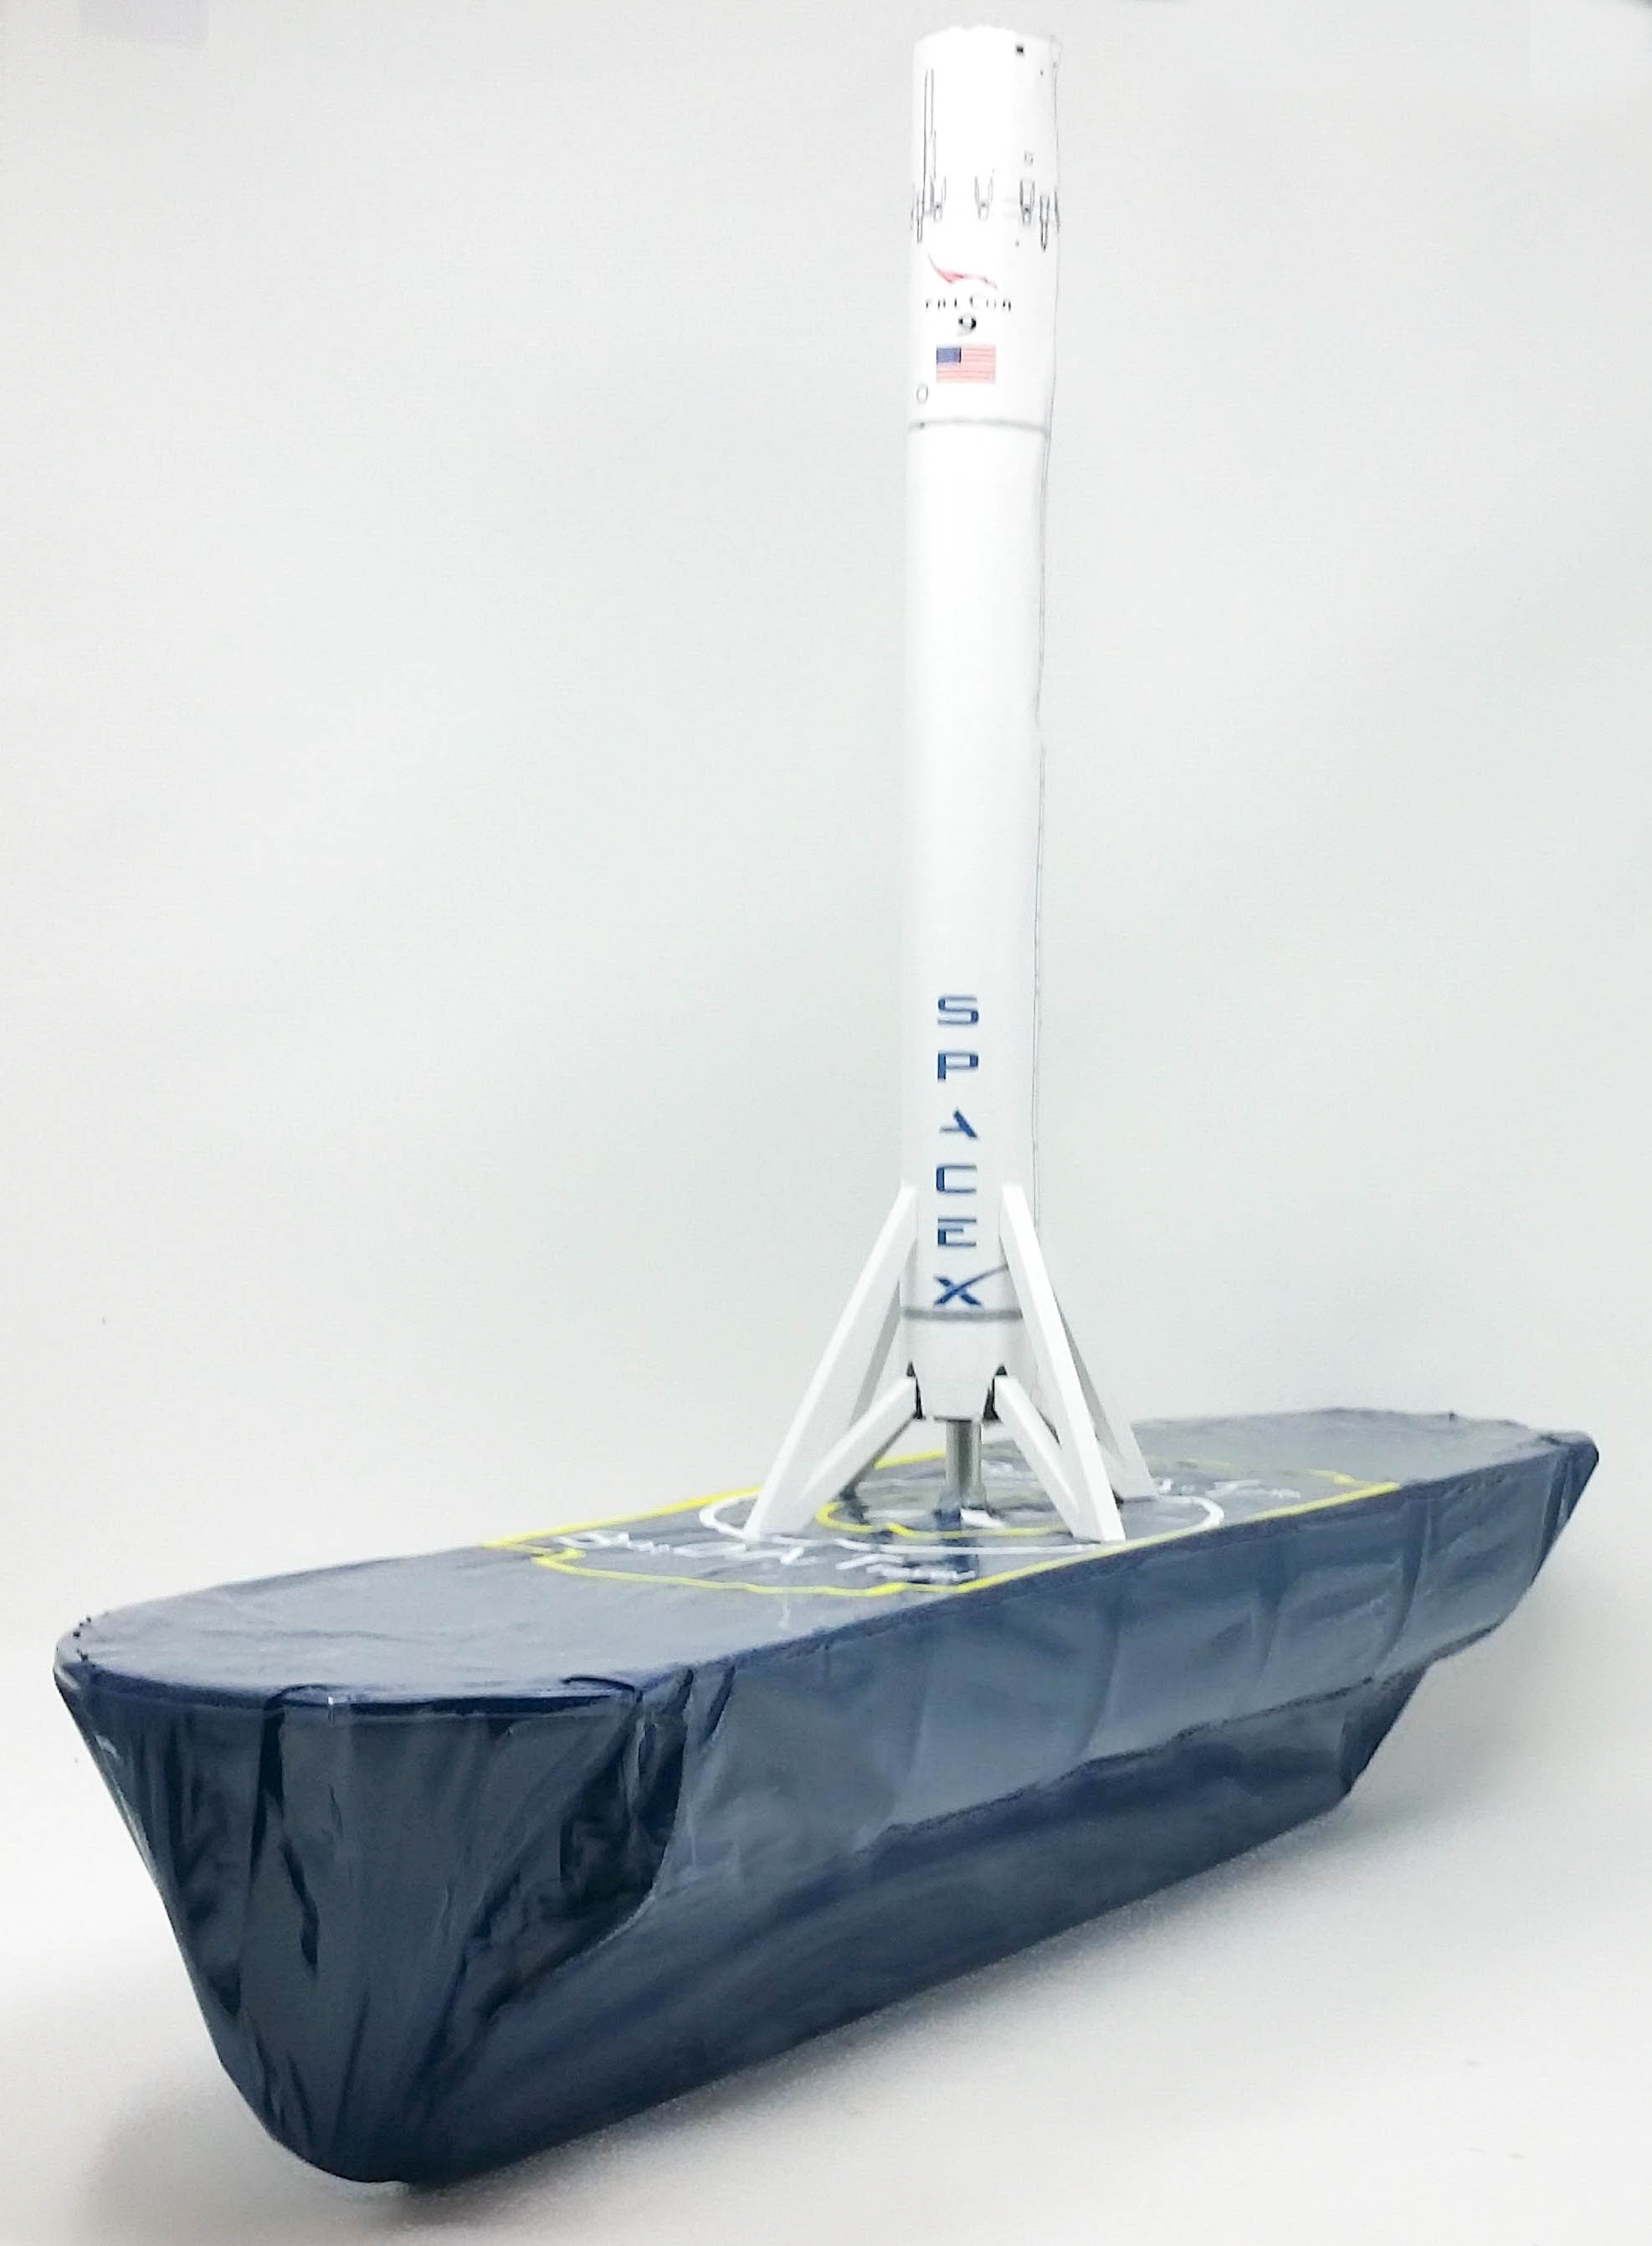
\includegraphics[width=0.15\textwidth]{FinishedBoat.jpg} &
    {Best Of All Time \newline Boat of Air Transportation}
    \end{tabularx}
  }

  \block{Performance Considerations}
  {
    \begin{itemize}
    \item The AVS should be \ang{130} to best fit between \ang{120} and \ang{140}.
    \item The boat will have little velocity, with a pulling force of \SI{.1}{\N}, so minimize the wet surface friction rather than wave breaking friction.
    \item The boat should be as long as possible to eliminate vortices.
    \end{itemize}
  }


  \column{0.6}
  \block{Righting Moment vs Heel Angle}{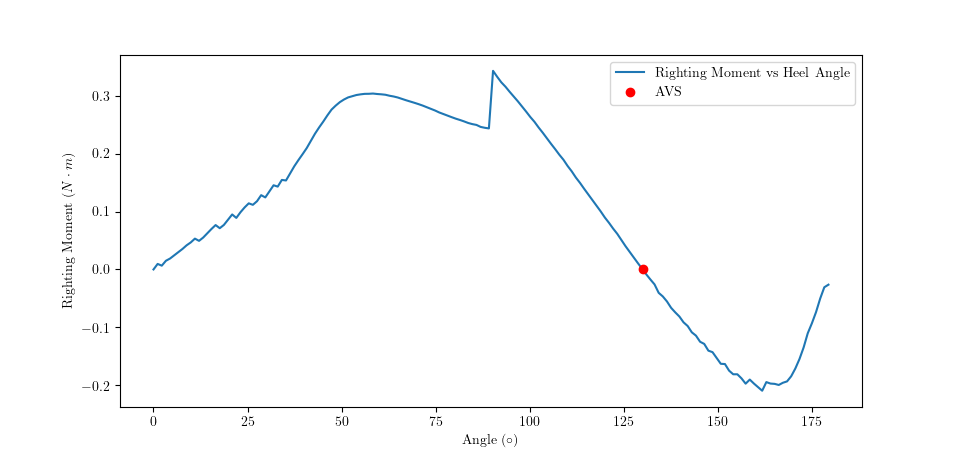
\includegraphics[width=0.53\textwidth]{curve.png}}


\end{columns}

\end{document}
